\documentclass[letterpaper,12pt]{article}
\usepackage[utf8]{inputenc}
\usepackage[T1]{fontenc}
\usepackage[top=0.8in,bottom=1.0in,left=0.75in,right=0.75in]{geometry}
\usepackage{mathptmx}
%\usepackage{fontspec} 
%\setmainfont{Times New Roman}
%\usepackage{color}
%\usepackage{array,ragged2e}
\usepackage{graphicx}
\usepackage[colorlinks=true, linkcolor=red]{hyperref}
%\usepackage{amsmath}
%\usepackage{titling,lipsum}
%\usepackage{booktabs}
%\usepackage{longtable}
\usepackage{float}
\usepackage{parskip}

\title{An FPGA Learning Experience:  SPI Interface to Max10 FPGA}
\author{Gregory Raven, KF5N \\ greg.electricity@gmail.com}

\begin{document}
	
		\maketitle
	
	\begin{abstract}
		A story of learning FPGA technology with the evolution of a simple project.
	\end{abstract}

\pagenumbering{gobble}

%\mainmatter
\section{Introduction}
%\pagenumbering{gobble}

This is the ``Golden Age'' of SBCs (Single Board Computers) and microcontroller boards.
Walk into your favorite brick-and-mortar bookstore (if you can find one), 
and check out the magazine shelf.  You will find several magazines, or ``book-a-zines''
dedicated to ``Arduino'' or ``Raspberry Pi''.  On the bookshelves you find a few books on Arduino and RPi, maybe even one for BeagleBone.

Or look in the magazine ''Make'', or use their ``Makers’ Guide to Boards'':

\url{https://makezine.com/comparison/boards/}

Using the above webpage, you can select a ``Type'' of board from three categories:

\begin{itemize}
	\item Microcontroller
	\item Single Board Computer
	\item FPGA
\end{itemize}

While there are dozens of boards listed, there are only three shown for ``FPGA''.
This list is not entirely accurate, as more FPGA boards o exist, however, it gives
an idea of the relative scarcity of FPGA boards.

There are a ton of resources online, and dozens of books and magazines on SBCs which you can find at the local bookstore.
The ARRL store sells several SBC themed books as well.  Do a search for FPGA.  Nothing!

I think it is fair to say that FPGA technology has not made it very far into the ranks of hobbyists.
Amateur radio experimenters have certainly been pioneers in FPGA, with numerous ``Software Defined Radio''
projects going back to the era when the devices were really expensive.  FPGA is an amazing technology, a sort of ``3D printer of digital electronics''.  Perhaps there are other applications of FPGA within the amateur radio world in addition to SDR which can be explored?

I wanted to experiment with this FPGA stuff! The current crop of devices and boards has lowered the cost of entry.  This is my story of a first project in FPGA.  Hopefully it can be shown that FPGA projects are within reach, and other hams can be encouraged to try working with this fascinating technology.

\section{Why?}

Why work with FPGAs?  Aren't SBCs good enough?

I like to think of FPGAs as a sort of ``3D printer for electronics''.  A loose analogy yes, but the point is that FPGAs allow you to create new digital circuits at will.  It is HARDWARE not software!  This gives you the power to create multiple specifically targeted digital machines which can work independently of one another.  This is the capability that SDR uses to crunch DSP math very efficiently while handling data flow simultaneously.  A list of FPGA applications from Wikipedia:

\url{https://en.wikipedia.org/wiki/Field-programmable_gate_array#Common_applications}

FPGAs will almost certainly be used in combination with conventional ``hard'' computing devices (like your laptop or Raspberry Pi).  Think of an FPGA as a capability you can add to your SBC to expand its capabilities into high-efficiency computing and the real-time domain.

\section{Where to Start}

When I began my FPGA quest, I was already familiar with the most common SBCs and microcontroller boards, the Arduino, the BeagleBone, and the Raspberry Pi.
It a good thing to have some experience developing with an SBC before attempting to tackle FPGA.  In my case, I spent quite a bit of time developing several projects on the BeagleBone Black.  Many of the skills learned working with SBCs will apply to FPGAs.

One of the ways I went up the learning curve on SBCs was this lecture series by Bruce Land of Cornell University:

\url{https://www.youtube.com/watch?v=FYy6JN0vpg0&list=PLKcjQ_UFkrd4z2qoFuJ1jtVhCSuxxCTpk}

This course uses a PIC32 microcontroller board.  However, the material in the lectures is generic enough to apply to any board which can be programmed in C.
Even better, a second course covers FPGA!

\url{https://www.youtube.com/playlist?list=PLKcjQ_UFkrd7UcOVMm39A6VdMbWWq-e_c}

and the matching website:

\url{http://people.ece.cornell.edu/land/courses/ece5760/}

Watching a few of the youtube videos gave me a pretty good idea of what was involved in FPGA work.
I didn't use the same development board as used in this course, but I did use
another Intel FPGA based board.  So the development tools and general flow of working
with the FPGA are similar.

You will need to use a variety of resources to answer questions and solve problems as you go up the FPGA learning curve.
It seemed to me that most of the effort required to learn FPGA is in handling a large quantity of details.
You will need to spend a lot of hours viewing videos, reading, and taking notes.  I think that FPGAs require at least a little more effort than working with SBCs.

\section{Your FPGA Manufacturer Web Site}

You will need to get an account at your FPGA manufacturer's website.  I used an Intel based board, and the account was free.
On the Intel site, you will have access to large amounts of learning resources for FPGA.
Be prepared to spend many hours watching videos and studying documentation, whatever FPGA you have chosen.
Intel has good material, and you can learn a lot!  A recommended starting point is the video series ``Become an FPGA Designer in 4 Hours''.
The 4 hours part is perhaps a bit optimistic, but it will give you a good early acceleration:

https://www.intel.com/content/www/us/en/programmable/support/training/course/odswbecome.html

\section{Github Repository for this Project}

The documentation and code for this project is located in this git repository:

\url{https://github.com/Greg-R/spiavalonfpga}
\section{Choosing a Development Board}

This was a not a straightforward process!

The first FPGA development board I purchased was the Numato Lab ``Elbert V2'' (\$29.95)
This board has the Xilinx XC3S50A Spartan 3A FPGA device containing 1584 logic cells and
54 KB RAM.  The board has a nice selection of peripherals which can be driven
by the FPGA:

\begin{itemize}
	\item 16 MB Flash Memory
	\item USB 2.0 interface for Flash programming
	\item 8 LEDs
	\item 6 push buttons
	\item DIP switch
	\item VGA connector
	\item Audio connector
	\item SD card adapter
	\item 3x 7 segment LED
	\item 39 IOs
\end{itemize}

Note that the USB capability of this board is for Flash programming only.  It is not an interface to the FPGA.

The reason for choosing the Elbert V2 was the book ``Programming FPGAs" by Simon Monk.  The book features the Elbert, along with the ``Mojo'' and ``Papilio'' boards.

It is interesting to note that a quick search on Amazon shows only three ``hobbyist'' style books for FPGA.
Contrast this to Arduino/Raspberry-Pi, where you will find dozens, maybe hundreds!

If you have a specific application, then it will be straightforward to decide if the development board meets your requirements.  For a person who is only interested in getting going in FPGA, then more peripheral devices are better than less.  Also note that the example above has 39 IOs, so you can add your own.  If the IO is in the format of the common Arduino, then adding peripherals may be quite easy to accomplish.

I was able to install the development software for the Elbert and work through a few of the projects in the book.
However, I found the development tools lacking in one area.  I was interested in using a more modern version of Verilog, called ``SystemVerilog''.  So that was a bit of a problem, and a search for another board began.

My motivation for SystemVerilog was to try some of the new features added, including those used for ``testbenches'' (simulation).  That is only an expression of my particular interest, as the Verilog used in the Xilinx tool for this device is fine and can be used for maximum benefit with this device.  This does, however, indicate that the development environment which mates up with the FPGA device is as important as the device itself.  So before you choose a board, be sure to download and install the development tools first.  Look at the documentation and decide if you will be comfortable with that particular development tool capabilities.

So looking around a bit more, I found this board after viewing Bruce Land's great lecture series on youtube:

\url{https://www.terasic.com.tw/cgi-bin/page/archive.pl?Language=English&CategoryNo=165&No=836}

The DE1-SOC is used in Cornell's ``ECE 5760 Advanced Microcontroller Design and system-on-chip'' course.

The board requires the "Quartus" development tool, which met my requirement for SystemVerilog.  However, this board is more complex than desired.  This board uses an advanced ''System On Chip'' (SOC) which is a combination of microcontroller (dual-core ARM Cortex A9) and FPGA in a single device.  Price is \$249, which seemed a little steep for a project which might not work out.  The added complexity of the ARM processors, having to deal with an unfamiliar distribution of Linux, and the extra work involved seemed like too much.  Indeed this board is immensely capable, so maybe I will come back to this one in the future!

Fortunately the same company, Terasic, makes board which are better suited to a beginner.  Perusing their site, I found this board, the DE10-Lite (\$85):

\url{https://www.terasic.com.tw/cgi-bin/page/archive.pl?Language=English&CategoryNo=234&No=1021}

This looked like a good choice, and it was purchased.  Later when doing internet searches, there was plenty of example projects already available for this board.  It seems to be at least moderately popular in the academic world, and some courses have been based on this board.  The MAX10 FPGA is widely supported, although it is not included in the latest version of the Quartus development tool (latest version supported 2018).

A good feature of this board is the Arduino compatible expansion header.  In general, the DE10-Lite has been easy to work with, and seems to be robust.  I've been using it for many months and it is still alive!




\section{A Project Inspiration: JTAG to FTDI SPI Interface}

The inspiration for this project came from a a search at github.com on DE10-Lite:

\url{https://github.com/hildebrandmw/de10lite-hdl}

This is a nice collection of work done with the DE10-Lite board for academic purposes.
What really got my attention is the project play\_gif:

\url{https://github.com/hildebrandmw/de10lite-hdl/tree/master/projects/play_gif}

The interesting feature of this project is the usage of the USB to load data (animated GIF image file)
to the FPGA.  So this is a data pipeline from a Linux desktop to the FPGA which is built into the board!
This met my requirement that I be able to control the FPGA remotely from a desktop (or SBC) computer.

The interface is via ``JTAG'', which is typically used as a debugging interface.  It is not specifically intended for mass data transfer, but in this case it was pressed into service.

The interface is a bit clunky to use.  It requires a ``TCL Server'', and a running instance of the Quartus development tool!  Not exactly what I was looking for, but I got the demo to work easily!  It is very nicely done work demonstrating several features of FPGA technology.

The way it works is conceptually simple.  The FPGA part of the project implements a VGA\footnote{VGA is a relatively simple video standard which seems to be common on many FPGA development boards.} interface to the connector on the DE10-Lite board.  The image loaded from the desktop computer is sliced into its constituent ``frames''.
Another interesting aspect of the project is the interface to the SDRAM of the DE10-Lite which is a 64MB external part on the board.  The sliced-up image is loaded into the SDRAM, and then another control module pages the VGA output through the memory.  Thus you see the animated GIF displayed on the monitor.  Really you are seeing in a very direct manner the data loaded into the SDRAM.  Cool!

\subsection{IP and Platform Designer}

First, a little bit of FPGA jargon.  ``Intellectual Property'' (IP) in the context of semiconductor devices is a block of circuitry which has been heavily engineered and refined to perform some particular function.  It could be patented or otherwise protected from duplication by competitors.
Due to the way integrated circuits are manufactured, blocks of ''IP'' can be added to the silicon and be expected to perform to the IP owner's specifications.  Typically IP can be included as part of a design kit, or it can be paid for with a license fee.

IP is good because it can reduce engineering design effort, improve performance, and enhance quality.  The trade-off is license fee cost, and you don't necessarily get exactly what you want.

In our case, we are given a whole bunch of IP for free that we can experiment with!  This is bundled into ``Platform Designer'' which is a tool-within-a-tool in the Quartus design suite.

To do justice to this there should be an entire section on ``Platform Designer''.  I will summarize here.  There are excellent video Platform Designer tutorials which you can access if you register for a free account at the Intel web site.

``Platform Designer'' is a building-block system.  You get a library of IP, along with a mechanism to hook them together.  The design is bundled into a ``Qsys'' file.    Let's have a look at the Qsys part of the play\_gif project:

\begin{figure}[h]
	\centering
	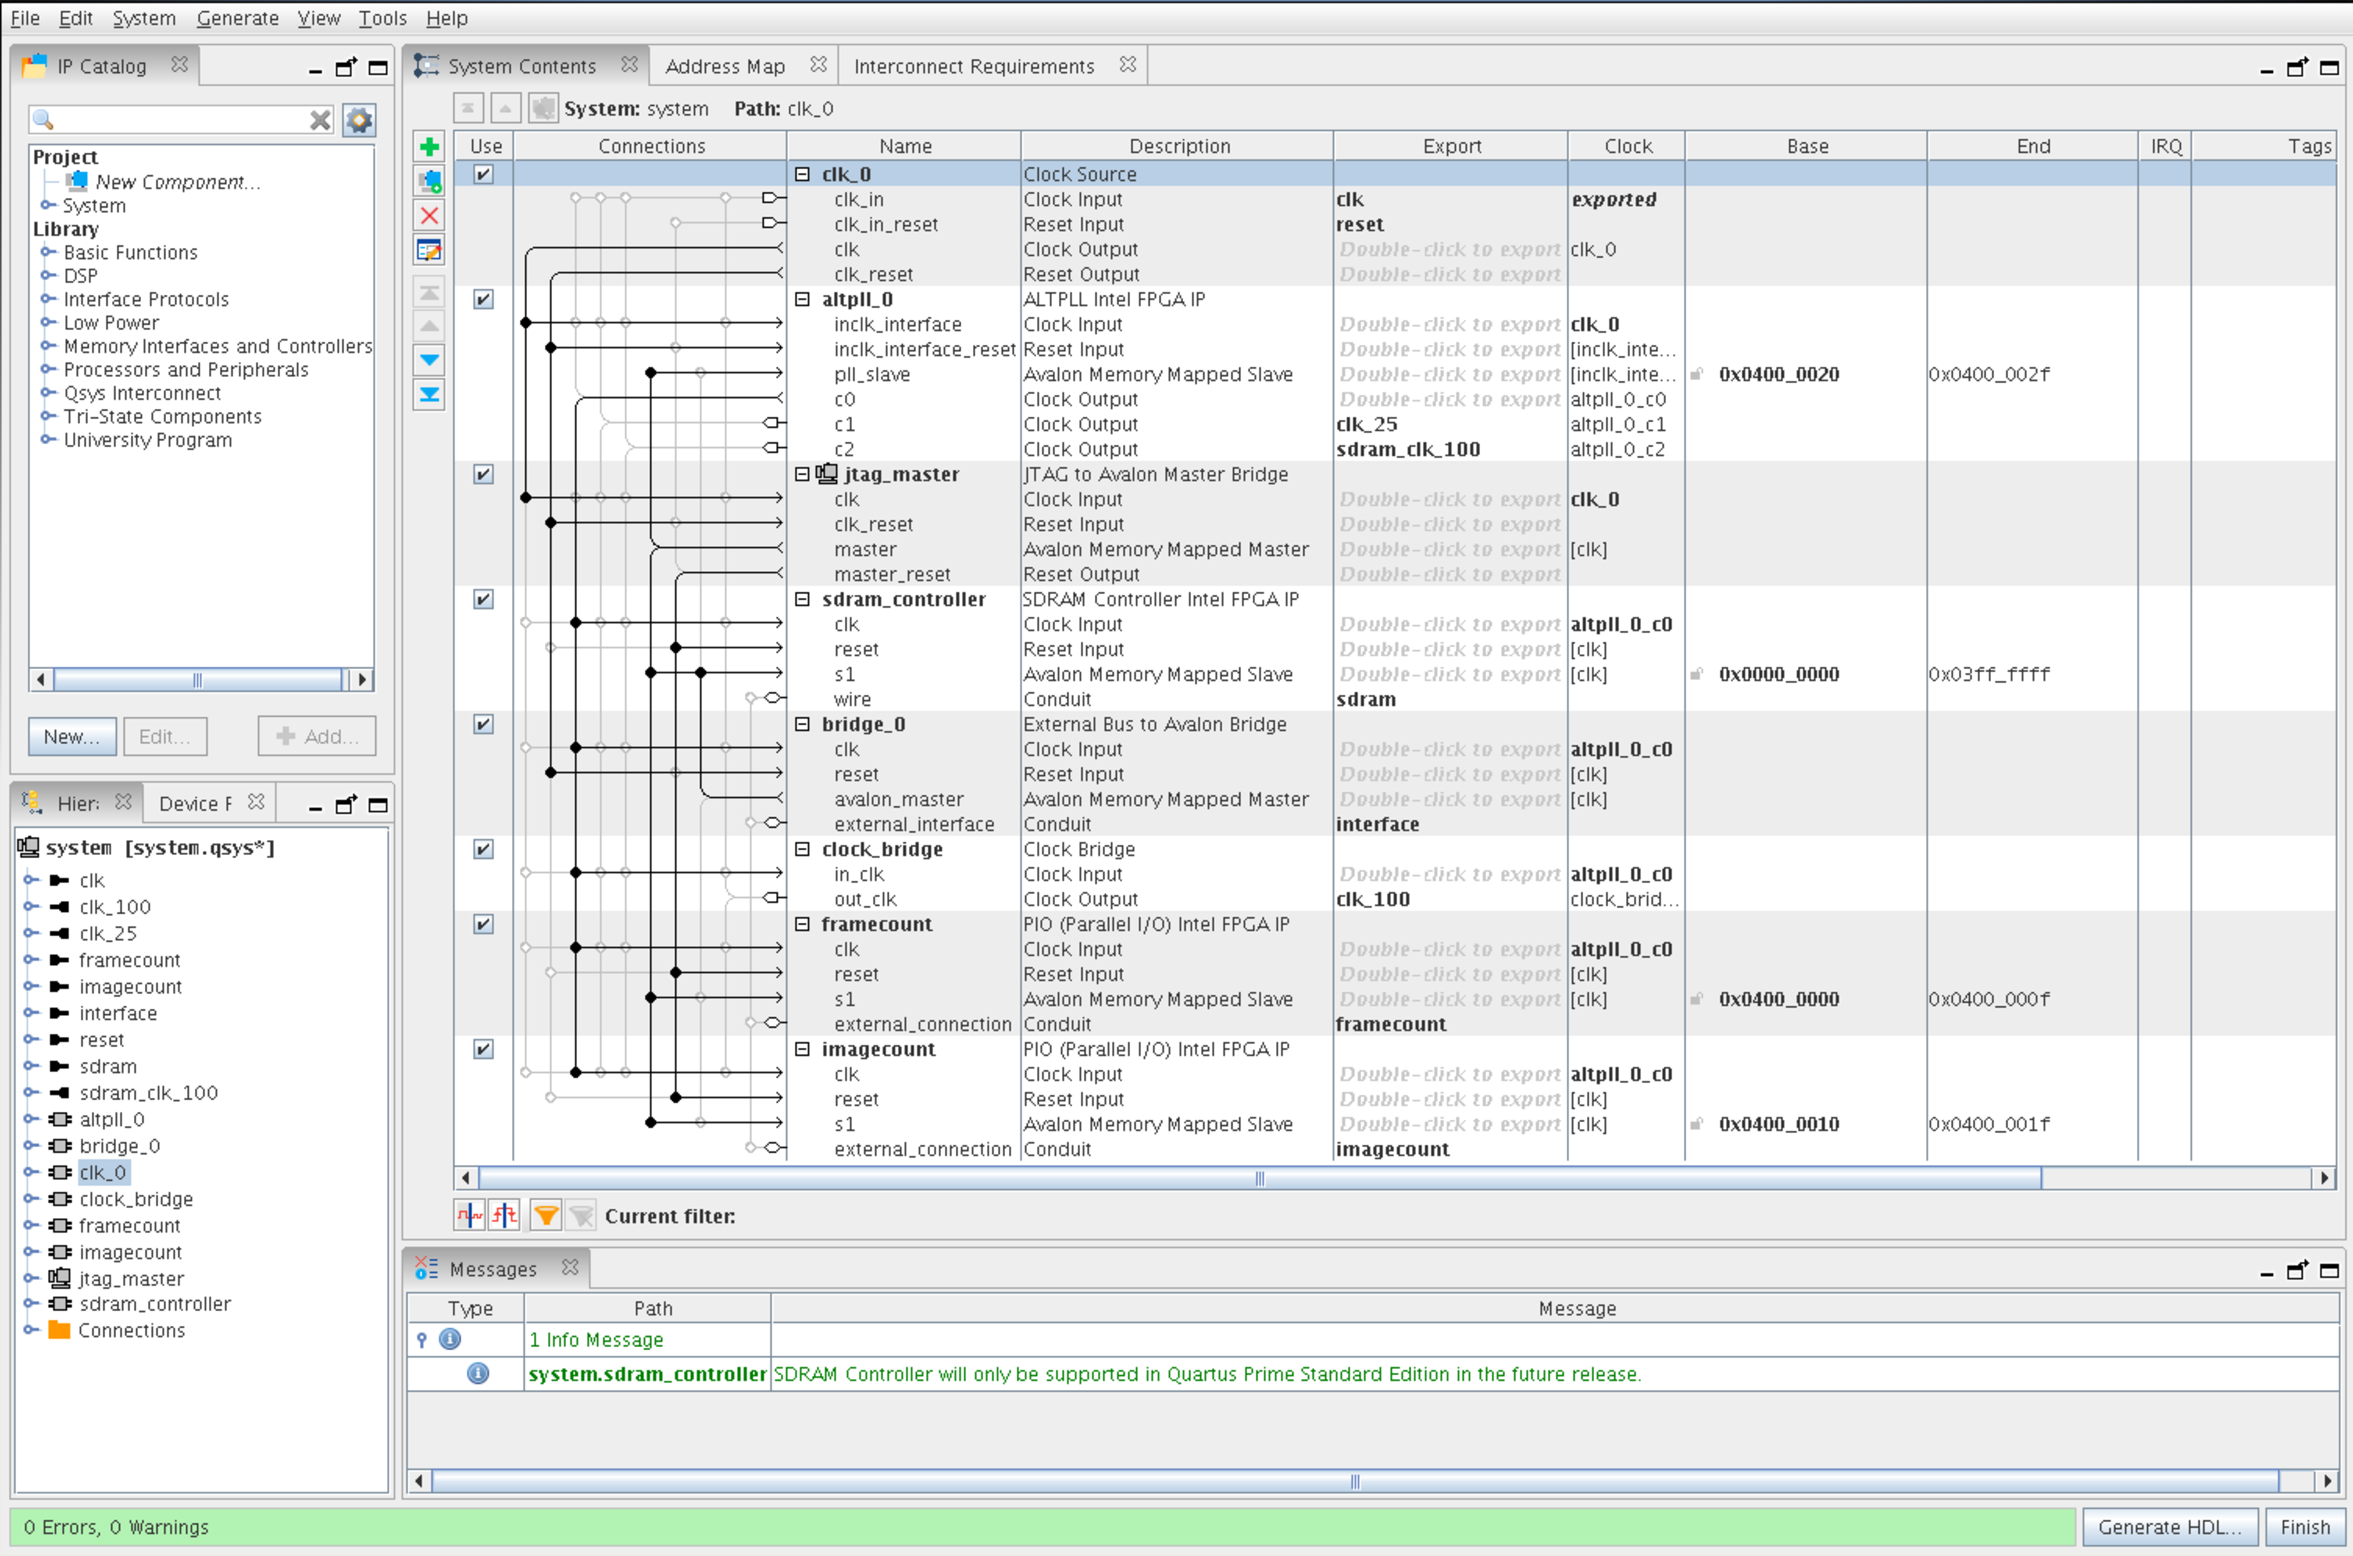
\includegraphics[width=1.0\textwidth]{images/platform_designer.pdf}
	\centering\bfseries
	\caption{Play\_gif project Qsys file}
\end{figure}

The upper left corner of the GUI is the library of IP.  Some of the categories:

\begin{itemize}
	\item Basic Functions
\item DSP
\item Memory Interfaces
\item Processors and Peripherals (including a ``Nios'' processor)
\item Memory Interfaces and Controllers
\end{itemize}

There is a sort of ``sub-library'' called  ``University Program'' which includes:

\begin{itemize}
	\item Audio and Video
\item Bridges
\item Clocks
\item Communication
\item Generic IO
\item Memory
\end{itemize}

The project used this IP:

\begin{enumerate}
\item ALTPLL Intel FPGA IP
\item JTAG to Avalon Master Bridge
\item DRAM Controller Intel FPGA IP
\item External Bus to Avalon Bridge
\item Clock Bridge
\item (Parallel IO) Intel FPGA IP
\end{enumerate}

The above IP can be seen in the column ``Name''.  There are two instantiations of the Parallel IO.
In the column ``Connections'' can be seen the graphical interconnections between the IP blocks.
Connections are made by simply clicking on the circles at the intersections of the ``wires'' between the IP.
Thus an entire system can be assembled using this GUI.  No writing of Verilog required!
The project does include some hand-written Verilog.  This ``Qsys'' design is ``dropped in'' to the project
as a Verilog module.

Here is what the system looks like:

\begin{figure}[h]
	\centering
	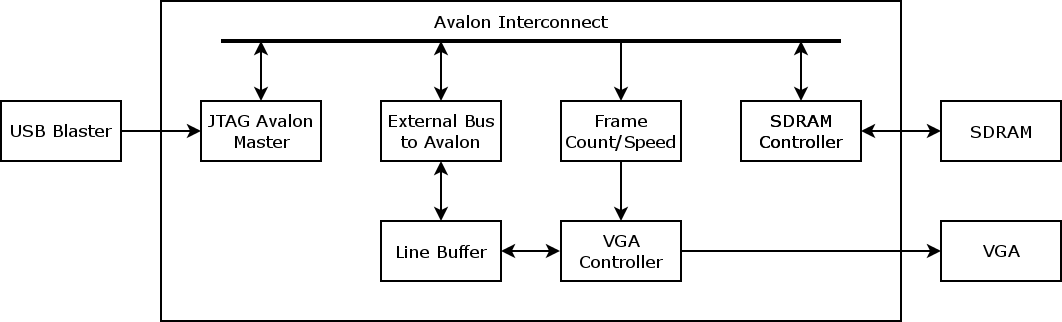
\includegraphics[width=1.0\textwidth]{images/play_gif.png}
	\centering\bfseries
	\caption{Play\_gif JTAG Interface System Diagram}
\end{figure}

What this diagram does not show is the requirement for a running Quartus and a TCL/JTAG server program.

The ``Avalon Interconnect'' deserves some explanation.  This is a system bus used in the MAX10 FPGA.  From the Avalon Interface specification:

\begin{quotation}
	Avalon® interfaces simplify system design by allowing you to easily connect
components in Intel® FPGA. The Avalon interface family defines interfaces appropriate
for streaming high-speed data, reading and writing registers and memory, and
controlling off-chip devices. Components available in Platform Designer incorporate
these standard interfaces. Additionally, you can incorporate Avalon interfaces in
custom components, enhancing the interoperability of designs.
\end{quotation}

It is an internal bus standard used to connect Avalon bus masters and slaves.  So it is a single-click process to connect Avalon components in Platform Designer.  It is really amazing what you get for such little effort!

This project is interesting, and shows a path to communication between a desktop computer and the FPGA.
However, the JTAG + Quartus + TCL/JTAG Server is cumbersome.  A SPI to Avalon bus IP component is listed in the catalog.
What if the JTAG and stuff could be replaced by something simpler like a SPI bus?

So that is what evolved into my ``introductory FPGA project''.  The revised system diagram:

\begin{figure}[h]
	\centering
	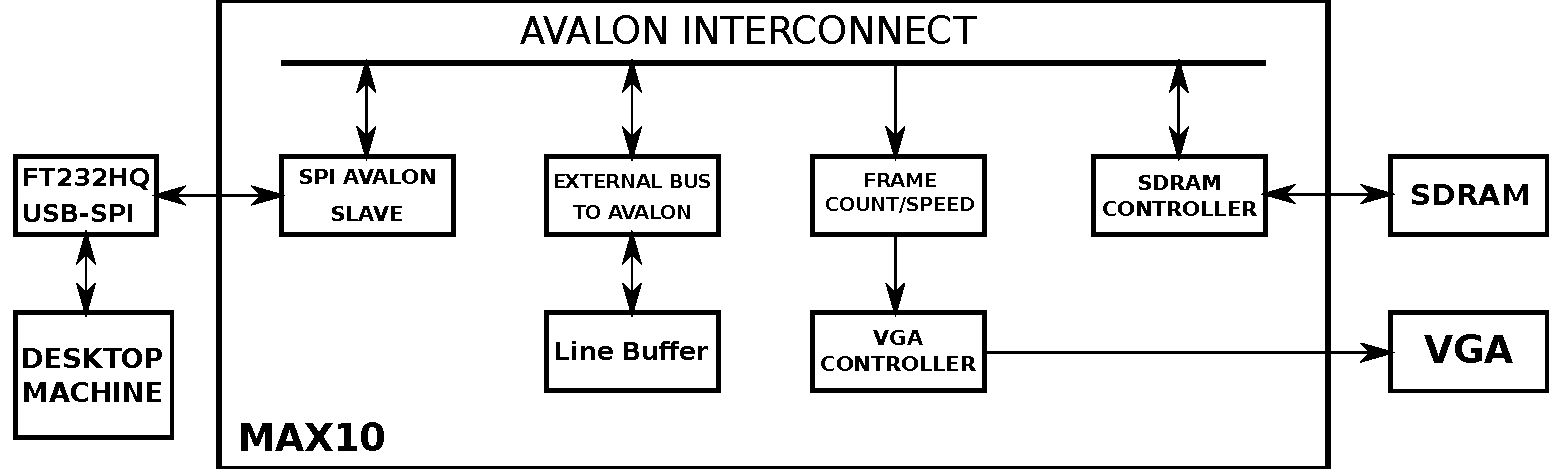
\includegraphics[width=1.0\textwidth]{images/spi_avalon_system}
	\centering\bfseries
	\caption{Play\_gif with SPI System Diagram}
\end{figure}

The significant change on the FPGA is the swapping of the JTAG Avalon bus master with the SPI-Avalon slave.  This was not entirely a drop-in replacement, as there were changes to reset and clock connections in addition to swapping JTAG to SPI components.  But it is easy, and the swapping can be done in a couple of minutes.

External to the DE10-Lite board, there is a USB to SPI adapter board.  This board is based on the FT232H chip by FTDI.  This can be bought from eBay for about \$10.  Search for ``ft232 spi'' and you will find several options.  I recommend one with headers to allow it to be plugged into a common breadboard.  The FTDI device requires a shared library (libMPSSE) to be installed:

\url{https://www.ftdichip.com/Support/SoftwareExamples/MPSSE/LibMPSSE-SPI.htm}

Other changes required for SPI:

\begin{itemize}
	\item The ports on the QSYS module changed (JTAG -> SPI), thus the Verilog module in which it is instantiated required minor changes.  This was done with the text editor feature of Quartus.
    \item Another change is required to the FPGA pins.  The new SPI bus must be routed to some easily accessible header on the DE10-Lite board.  Since the board has an Arduino compatible header, and this header has a standard set of four pins for SPI, those pins were used.  The details can be seen in the DE10-Lite manual provided by Terasic.  The ``Pin Planner'' tool was used to make the changes.
    \item The ``Synopsys Design Constraints'' (.sdc) file was updated to incorporate the SPI bus.
\end{itemize}

Here is the crazy breadboard hook-up:

\begin{figure}[h]
	\centering
	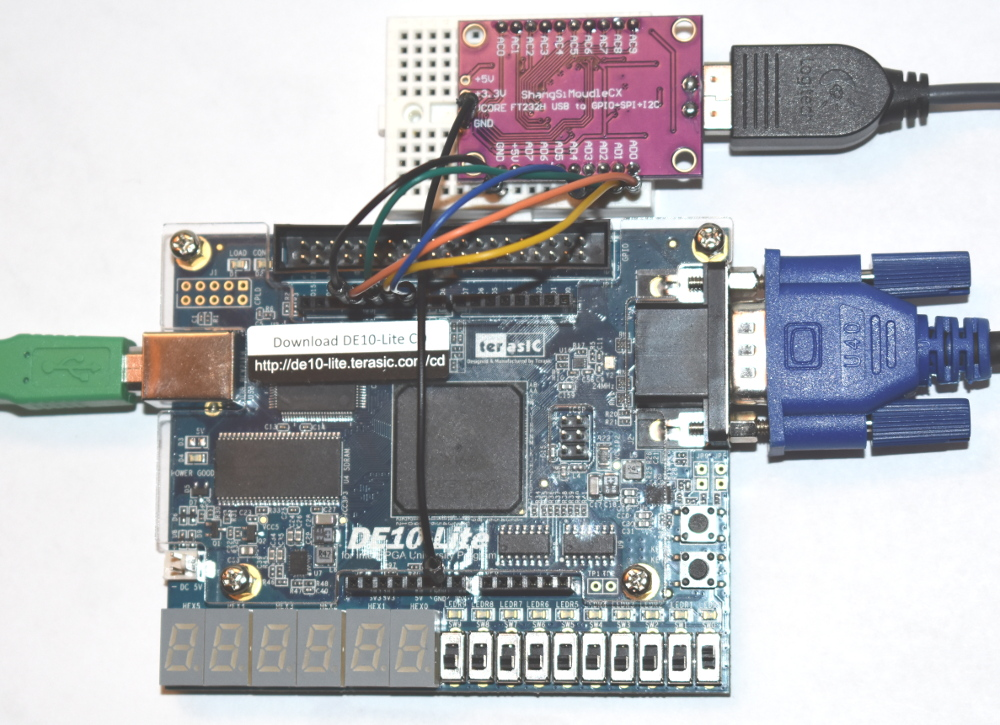
\includegraphics[width=0.5\textwidth]{images/de10_spi}
	\centering\bfseries
	\caption{DE10-Lite Connected to FTDI SPI Breakout}
\end{figure}

In spite of the length of the breadboard jumper wires, the SPI interface performed remarkably well right up to the FTDI clock limit of 30 MHz.










\section{SPI Driver in Julia Programming Language}

The github project from which mine was derived uses a programming language called ``Julia'':

\url{https://julialang.org/}

This was a language I had heard about, but I've never tried it.
To duplicate the original project, I had to install the language and run the program.
The program does the processing of the GIF image, and then sends the data to the FPGA
via the JTAG server and USB-to-JTAG interface.

It was simple to install the server and run the Julia program.  It all worked first time!
Later, I installed the Atom IDE which has a Julia plug-in.  It's great!

Rather than reinventing the wheel, I decided to use the image processing portion of the Julia program.
However, how to drive the FTDI SPI device?  I needed something to replace the JTAG server.

The FTDI USB-to-SPI device is supported with a C shared library.  This library has the initialization, read, write, and shutdown
command necessary to work with the device.

Fortuitously, the Julia language includes the capability to call C library functions in a very direct way!
I was skeptical at first, but I quickly had the SPI device's initialization function running and returning with no error.
The other required functions were quickly added.  I now had full control of the SPI bus from the command line!

When I say ``command line'', in the case of Julia I am referring to the ``Read Eval Print Loop'', called the REPL.  This functionality is similar to Python, and is my favorite way to develop code.  I also used the ``Atom'' IDE, which has a plug-in for the Julia language.
It is a new language, and has a few quirks like all of them do, but so far I am very impressed!

At first, Julia was also used to access a shared library which was taken from an Altera demo project of the SPI-Avalon bus master.
This library was responsible for reading and writing ``Avalon Packets''.  This is the protocol used by the Avalon bus.  I was able to successfully translate the Altera library to Julia.  This is working well and the system is able to read and write to the SPI and thus the FPGA Avalon bus, the parallel ports, and the SDRAM.

\begin{figure}[ht]
	\centering
	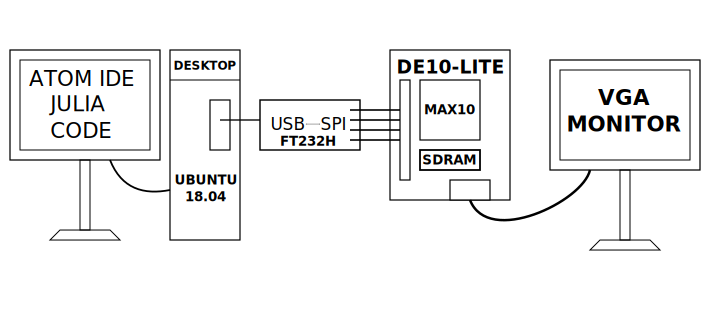
\includegraphics[width=0.7\textwidth]{images/project_system}
	\centering\bfseries
	\caption{Project System:  Desktop -> USB-to-SPI -> FPGA -> VGA Monitor}
\end{figure}

The Julia code is located in the ``julia'' directory of the github repository linked in the introduction.

\section{FPGA and Verilog Books}

\subsection{Hobbyist FPGA Books}

"Designing Video Game Hardware in Verilog"
Steven Hugg, first printing 2018

A very practical introduction to digital hardware using the early history of video games as a means of illustrating the technology.
The book includes significant introduction to Verilog and its relationship to the physical circuitry.

However, it is not primarily an FPGA book!  The reader is encouraged to use a web-based Verilog simulator:

\url{http://8bitworkshop.com}

There is an example FPGA which uses the iCE40HX-1K iCEstick.
This is a low-cost device (\$40 on Amazon).  Development can proceed
with the official Lattice tool chain, or with an open-source system
known as ``IceStorm'':

\url{http://www.clifford.at/icestorm}

``Programming FPGAs, Getting Started in Verilog''
Simon Monk, 2017 McGraw-Hill Education

Good coverage of beginning FPGA using the boards Elbert 2, Mojo, and Papilio.

\url{https://www.amazon.com/Programming-FPGAs-Getting-Started-Verilog/dp/125964376X/ref=sr_1_1?keywords=fpga+monk&qid=1564448368&s=books&sr=1-1}

\subsection{Verilog}

You will need to go up the learning curve on Verilog (or VHDL).
Here are a couple of inexpensive books (< \$20) which will get you going:

``Designing Digital Systems with SystemVerilog''
Brent E. Nelson, Brigham Young University

\url{https://www.amazon.com/gp/product/1075968437/ref=ppx_yo_dt_b_asin_title_o00_s03?ie=UTF8&psc=1}

``Exploring Digital Logic''
George Self.

\url{http://www.lulu.com/shop/george-self/exploring-digital-logic/paperback/product-22747579.html}

Free eBook by Intel:

``FPGAs for Dummies''

\url{https://plan.seek.intel.com/PSG_WW_NC_LPCD_FR_2018_FPGAforDummiesbook}


\section{Simulation}

The FPGA developer should develop skills in FPGA simulation.  The ``blinky LED'' project I attempted prior to the SPI bus project required me to do that.
I had a minor, but persistent bug which brought my work to a halt.  Trial and error with the board and re-doing the FPGA got me nowhere fast.  After I had a simple simulation running, the problem was quickly resolved.
Fortunately the Quartus tool does most of the work to set up the simulation.  A small bit of hacking of ``do'' (TCL) files is required.

I recommend using the resources on the Intel web site to explore the basics of setting up and running simulations via Quartus.

\section{Conclusion}

I was able to find an FPGA development board and ``starter project'' that met my requirements for a beginning in FPGA development.
A bare minimum of Verilog modifications were required to make the project function correctly.

Most of the FPGA ``design'' was done using the system-level ``Platform Designer'' tool.

I was able to add memory-mapped read of the SDRAM and FPGA registers via analysis of the Avalon bus structure.  The Julia programming
language was used to create and decode Avalon bus transactions.  Direct access of the SPI device C shared library from Julia code was used.

The next stage of the project will be a practical ham radio application.  I have an antenna rotator which I want to control via wireless.
I think it will be possible to create a real-time state machine on the FPGA which will handle the motor drive along with a Hall sensor
and counter for positional feedback.  Driving the FPGA from the SPI port of an SBC, along with a WIFI connection, should allow the entire
control unit to be wireless.  Solar powered?  Maybe.



\end{document}